\documentclass[12pt]{article}
\usepackage{geometry}
\usepackage{subfig}
\usepackage{graphicx,graphics,epsfig,subfigure,times,bm,bbm,amssymb,amsmath,amsfonts,amsthm,amscd,mathrsfs,MnSymbol,accents}
\usepackage[matrix,frame,arrow]{xypic}
\usepackage[pdftex]{color}

\usepackage{braket}%Dirac Notation in QM
\usepackage{enumerate}
%    Q-circuit version 1.2
%    Copyright (C) 2004  Steve Flammia & Bryan Eastin, 4/23/06
%    This program is free software; you can redistribute it and/or modify
%    it under the terms of the GNU General Public License as published by
%    the Free Software Foundation; either version 2 of the License, or
%    (at your option) any later version.
%
%    This program is distributed in the hope that it will be useful,
%    but WITHOUT ANY WARRANTY; without even the implied warranty of
%    MERCHANTABILITY or FITNESS FOR A PARTICULAR PURPOSE.  See the
%    GNU General Public License for more details.
%
%    You should have received a copy of the GNU General Public License
%    along with this program; if not, write to the Free Software
%    Foundation, Inc., 59 Temple Place, Suite 330, Boston, MA  02111-1307  USA

\usepackage[matrix,frame,arrow]{xy}
\usepackage{amsmath}
\newcommand{\bra}[1]{\left\langle{#1}\right\vert}
\newcommand{\ket}[1]{\left\vert{#1}\right\rangle}
    % Defines Dirac notation.
\newcommand{\qw}[1][-1]{\ar @{-} [0,#1]}
    % Defines a wire that connects horizontally.  By default it connects to the object on the left of the current object.
    % WARNING: Wire commands must appear after the gate in any given entry.
\newcommand{\qwx}[1][-1]{\ar @{-} [#1,0]}
    % Defines a wire that connects vertically.  By default it connects to the object above the current object.
    % WARNING: Wire commands must appear after the gate in any given entry.
\newcommand{\cw}[1][-1]{\ar @{=} [0,#1]}
    % Defines a classical wire that connects horizontally.  By default it connects to the object on the left of the current object.
    % WARNING: Wire commands must appear after the gate in any given entry.
\newcommand{\cwx}[1][-1]{\ar @{=} [#1,0]}
    % Defines a classical wire that connects vertically.  By default it connects to the object above the current object.
    % WARNING: Wire commands must appear after the gate in any given entry.
\newcommand{\gate}[1]{*{\xy *+<.6em>{#1};p\save+LU;+RU **\dir{-}\restore\save+RU;+RD **\dir{-}\restore\save+RD;+LD **\dir{-}\restore\POS+LD;+LU **\dir{-}\endxy} \qw}
    % Boxes the argument, making a gate.
\newcommand{\meter}{\gate{\xy *!<0em,1.1em>h\cir<1.1em>{ur_dr},!U-<0em,.4em>;p+<.5em,.9em> **h\dir{-} \POS <-.6em,.4em> *{},<.6em,-.4em> *{} \endxy}}
    % Inserts a measurement meter.
\newcommand{\measure}[1]{*+[F-:<.9em>]{#1} \qw}
    % Inserts a measurement bubble with user defined text.
\newcommand{\measuretab}[1]{*{\xy *+<.6em>{#1};p\save+LU;+RU **\dir{-}\restore\save+RU;+RD **\dir{-}\restore\save+RD;+LD **\dir{-}\restore\save+LD;+LC-<.5em,0em> **\dir{-} \restore\POS+LU;+LC-<.5em,0em> **\dir{-} \endxy} \qw}
    % Inserts a measurement tab with user defined text.
\newcommand{\measureD}[1]{*{\xy*+=+<.5em>{\vphantom{\rule{0em}{.1em}#1}}*\cir{r_l};p\save*!R{#1} \restore\save+UC;+UC-<.5em,0em>*!R{\hphantom{#1}}+L **\dir{-} \restore\save+DC;+DC-<.5em,0em>*!R{\hphantom{#1}}+L **\dir{-} \restore\POS+UC-<.5em,0em>*!R{\hphantom{#1}}+L;+DC-<.5em,0em>*!R{\hphantom{#1}}+L **\dir{-} \endxy} \qw}
    % Inserts a D-shaped measurement gate with user defined text.
\newcommand{\multimeasure}[2]{*+<1em,.9em>{\hphantom{#2}} \qw \POS[0,0].[#1,0];p !C *{#2},p \drop\frm<.9em>{-}}
    % Draws a multiple qubit measurement bubble starting at the current position and spanning #1 additional gates below.
    % #2 gives the label for the gate.
    % You must use an argument of the same width as #2 in \ghost for the wires to connect properly on the lower lines.
\newcommand{\multimeasureD}[2]{*+<1em,.9em>{\hphantom{#2}}\save[0,0].[#1,0];p\save !C *{#2},p+LU+<0em,0em>;+RU+<-.8em,0em> **\dir{-}\restore\save +LD;+LU **\dir{-}\restore\save +LD;+RD-<.8em,0em> **\dir{-} \restore\save +RD+<0em,.8em>;+RU-<0em,.8em> **\dir{-} \restore \POS !UR*!UR{\cir<.9em>{r_d}};!DR*!DR{\cir<.9em>{d_l}}\restore \qw}
    % Draws a multiple qubit D-shaped measurement gate starting at the current position and spanning #1 additional gates below.
    % #2 gives the label for the gate.
    % You must use an argument of the same width as #2 in \ghost for the wires to connect properly on the lower lines.
\newcommand{\control}{*!<0em,.025em>-=-{\bullet}}
    % Inserts an unconnected control.
\newcommand{\controlo}{*-<.21em,.21em>{\xy *=<.59em>!<0em,-.02em>[o][F]{}\POS!C\endxy}}
    % Inserts a unconnected control-on-0.
\newcommand{\ctrl}[1]{\control \qwx[#1] \qw}
    % Inserts a control and connects it to the object #1 wires below.
\newcommand{\ctrlo}[1]{\controlo \qwx[#1] \qw}
    % Inserts a control-on-0 and connects it to the object #1 wires below.
\newcommand{\targ}{*!<0em,.019em>=<.79em,.68em>{\xy {<0em,0em>*{} \ar @{ - } +<.4em,0em> \ar @{ - } -<.4em,0em> \ar @{ - } +<0em,.36em> \ar @{ - } -<0em,.36em>},<0em,-.019em>*+<.8em>\frm{o}\endxy} \qw}
    % Inserts a CNOT target.
\newcommand{\qswap}{*=<0em>{\times} \qw}
    % Inserts half a swap gate. 
    % Must be connected to the other swap with \qwx.
\newcommand{\multigate}[2]{*+<1em,.9em>{\hphantom{#2}} \qw \POS[0,0].[#1,0];p !C *{#2},p \save+LU;+RU **\dir{-}\restore\save+RU;+RD **\dir{-}\restore\save+RD;+LD **\dir{-}\restore\save+LD;+LU **\dir{-}\restore}
    % Draws a multiple qubit gate starting at the current position and spanning #1 additional gates below.
    % #2 gives the label for the gate.
    % You must use an argument of the same width as #2 in \ghost for the wires to connect properly on the lower lines.
\newcommand{\ghost}[1]{*+<1em,.9em>{\hphantom{#1}} \qw}
    % Leaves space for \multigate on wires other than the one on which \multigate appears.  Without this command wires will cross your gate.
    % #1 should match the second argument in the corresponding \multigate. 
\newcommand{\push}[1]{*{#1}}
    % Inserts #1, overriding the default that causes entries to have zero size.  This command takes the place of a gate.
    % Like a gate, it must precede any wire commands.
    % \push is useful for forcing columns apart.
    % NOTE: It might be useful to know that a gate is about 1.3 times the height of its contents.  I.e. \gate{M} is 1.3em tall.
    % WARNING: \push must appear before any wire commands and may not appear in an entry with a gate or label.
\newcommand{\gategroup}[6]{\POS"#1,#2"."#3,#2"."#1,#4"."#3,#4"!C*+<#5>\frm{#6}}
    % Constructs a box or bracket enclosing the square block spanning rows #1-#3 and columns=#2-#4.
    % The block is given a margin #5/2, so #5 should be a valid length.
    % #6 can take the following arguments -- or . or _\} or ^\} or \{ or \} or _) or ^) or ( or ) where the first two options yield dashed and
    % dotted boxes respectively, and the last eight options yield bottom, top, left, and right braces of the curly or normal variety.
    % \gategroup can appear at the end of any gate entry, but it's good form to pick one of the corner gates.
    % BUG: \gategroup uses the four corner gates to determine the size of the bounding box.  Other gates may stick out of that box.  See \prop. 
\newcommand{\rstick}[1]{*!L!<-.5em,0em>=<0em>{#1}}
    % Centers the left side of #1 in the cell.  Intended for lining up wire labels.  Note that non-gates have default size zero.
\newcommand{\lstick}[1]{*!R!<.5em,0em>=<0em>{#1}}
    % Centers the right side of #1 in the cell.  Intended for lining up wire labels.  Note that non-gates have default size zero.
\newcommand{\ustick}[1]{*!D!<0em,-.5em>=<0em>{#1}}
    % Centers the bottom of #1 in the cell.  Intended for lining up wire labels.  Note that non-gates have default size zero.
\newcommand{\dstick}[1]{*!U!<0em,.5em>=<0em>{#1}}
    % Centers the top of #1 in the cell.  Intended for lining up wire labels.  Note that non-gates have default size zero.
\newcommand{\Qcircuit}[1][0em]{\xymatrix @*[o] @*=<#1>}
    % Defines \Qcircuit as an \xymatrix with entries of default size 0em.  The optional argument, #1, is for use with clusters, and allows you
    % to fix the size of the nodes.  I would not advise using it with normal circuits.
\newcommand{\node}[2][]{{\begin{array}{c} \ _{#1}\  \\ {#2} \\ \ \end{array}}\drop\frm{o} }
    % When Qcircuit has been passed the optional argument for cluster states, this command produces a round node of the size specified in that
    % argument.  The optional argument #2 specifies the contents of a node, while optional argument #1 is a secondary label.  
\newcommand{\link}[2]{\ar @{-} [#1,#2]}
    % Draws a wire or connecting line to the element #1 rows down and #2 columns forward.
\newcommand{\pureghost}[1]{*+<1em,.9em>{\hphantom{#1}}}
    % Same as \ghost except it omits the wire leading to the left.  %Quantum Circuits
\usepackage{multirow}
\usepackage{textcomp}
\usepackage{booktabs}
\usepackage[english]{babel}
\usepackage{url}
\usepackage{appendix}
\usepackage[counter-within=section,counter-format=ch.se.qu]{exsheets}
\usepackage{makeidx}
\usepackage[pdfstartview=FitH]{hyperref}
\hypersetup{
    colorlinks=true,       % false: boxed links; true: colored links
    linkcolor=cyan,          % color of internal links
    citecolor=magenta,        % color of links to bibliography
    filecolor=magenta,      % color of file links
    urlcolor=cyan,           % color of external links
    runcolor=cyan
}
\usepackage[capitalise]{cleveref}
\usepackage{cancel}
\usepackage{mathtools}

\renewcommand*{\theHsection}{\thesection}
\renewcommand*{\theHsubsection}{\thesubsection}
\usepackage{hypernat}
\usepackage{environ}
\usepackage{ragged2e}
\usepackage{caption}



% Define a new environment for tables with customized captions
\newenvironment{mytable}
  {% Begin code
   \begin{table}[ht]
   \centering
  }
  {% End code
   \end{table}
  }

%% Override the caption formatting of cup6a
\makeatletter
\long\def\make@table@caption#1#2{\vskip 10\p@%
    \setbox\@tempboxa\hbox{{\rm #1.\hspace{0.5em}\itshape #2}}%
    \ifdim \wd\@tempboxa >\hsize
    { \rm #1.\hspace{0.5em}{\itshape #2}\par}%
    \else
    \ifSFB@indentsty
    \hbox to\hsize{\box\@tempboxa\hfill}\par
    \else
    \hbox to\hsize{\hfil\box\@tempboxa\hfil}\par
    \fi
    \fi
    \vspace*{2.5\p@}\par
}
\makeatother

% Custom command to create a caption with specific formatting
\newcommand{\mycaption}[1]{%
  \caption{%
     #1
}%
}

\makeindex

\usepackage{paralist} 
\usepackage{psfrag} 
\usepackage{cupbookpatch11}
\usepackage{color}
\usepackage{fancyhdr}
\usepackage[PetersLenny]{fncychap}
\usepackage{tikz}
\usetikzlibrary{positioning}
\def\checkmark{\tikz\fill[scale=0.4](0,.35) -- (.25,0) -- (1,.7) -- (.25,.15) -- cycle;}

\setlength{\unitlength}{1cm}

\setlength{\marginparwidth}{1.5in}
\setlength{\textheight}{9.5in}
\setlength{\textwidth}{6in}
\setlength{\topmargin}{-.5in}
\setlength{\oddsidemargin}{.16in}
\setlength{\evensidemargin}{.2in} 
\setlength{\headsep}{.5in} 
\setlength{\parindent}{1.5pc}

\renewcommand{\baselinestretch}{1.02}
\newcommand{\HRule}{\hskip -.6cm \rule{\linewidth}{0.2mm}}

%superscript footnote
\makeatletter
\def\@makefnmark{\hbox{\@textsuperscript{\normalfont\@thefnmark}}}
\makeatother

% for algorithms
\usepackage{algorithm}
\usepackage{algpseudocode}

\newtheorem{thm}{Theorem}[section]
\newtheorem{mydef}{Definition}[section]
\newtheorem{col}{Corollary}[section]
\newtheorem{pos}{Postulate}[section]

\newtheorem{mytheorem}{Theorem}[section]
\newtheorem{mylemma}{Lemma}[section]
\newtheorem{mycorollary}{Corollary}[section]
\newtheorem{myproposition}{Proposition}[section]
\newtheorem{myclaim}{Claim}[section]
\newtheorem{mydefinition}{Definition}[section]
\newtheorem{myassumption}{Assumption}[section]
\newtheorem{mypostulate}{Postulate}[]

% Primed postulates
\makeatletter
\newcommand{\neutralize}[1]{\expandafter\let\csname c@#1\endcsname\count@}
\makeatother

\newenvironment{mypostulateDM}[1]
{\renewcommand{\thepos}{\ref*{#1}$'$}%
    \neutralize{ps}\phantomsection%
    \begin{pos}}%
    {\end{pos}}%

\newenvironment{mypostulateDM2}[1]
{\renewcommand{\thepos}{\ref*{#1}$''$}%
    \neutralize{ps}\phantomsection%
    \begin{pos}}%
    {\end{pos}}%

\newcommand{\msf}{\mathsf}
\newcommand{\mrm}{\mathrm}
\newcommand{\mbf}{\mathbf}
\newcommand{\mbb}{\mathbb}
\newcommand{\mc}{\mathcal}
\newcommand{\tx}[1]{\text{#1}}
\newcommand{\derv}[3]{\frac{d^{#3}#1}{d#2^{#3}}}					% DERIVATIVE
\newcommand{\pdv}[2]{\frac{\partial#1}{\partial#2}}
\newcommand{\half}{\tfrac{1}{2}}

\newcommand{\bes} {\begin{subequations}}
\newcommand{\ees} {\end{subequations}}
\newcommand{\ba}{\begin{eqnarray}}
\newcommand{\ea}{\end{eqnarray}}
\newcommand{\bea} {\begin{eqnarray}}
\newcommand{\eea} {\end{eqnarray}}
\newcommand{\beq}{\begin{equation}}
\newcommand{\eeq}{\end{equation}}


\newcommand{\red}[1]{\textcolor{red}{#1}} 
\newcommand{\green}[1]{\textcolor{black}{#1}}
\newcommand{\blue}[1]{\textcolor{blue}{#1}}

\newcommand{\expv}[1]{\langle #1\rangle}							% EXPECTATION VALUE
\newcommand{\ph}{\ensuremath{\varphi}}
\newcommand{\eps}{\ensuremath{\varepsilon}} %"nice" epsilon
\newcommand{\prima}[1]{\ensuremath{#1^\prime}} %add a prime to something
\newcommand{\R}{\ensuremath{\mathbb{R}}} %real numbers
\newcommand{\C}{\ensuremath{\mathbb{C}}} %complex numbers
\newcommand{\Q}{\ensuremath{\mathbb{Q}}} %rational numbers
\newcommand{\Z}{\ensuremath{\mathbb{Z}}} %integers
\newcommand{\N}{\ensuremath{\mathbb{N}}} %natural numbers
\newcommand{\e}{\ensuremath{{e}}} %e:=lim_{n\to\infty}(1+1/n)^n
\newcommand{\ii}{\ensuremath{{i}}}%i:=\sqrt{-1}
\newcommand{\abs}[1]{\ensuremath{\left|#1\right|}} %absolute value
\newcommand{\norm}[1]{\ensuremath{\left\|#1\right\|}} %norm
\newcommand{\opU}{\ensuremath{{{U}}}}
\newcommand{\opH}{\ensuremath{{{H}}}}
\newcommand{\dfsh}{\mathrm{DFS}}
\newcommand{\mcal}[1]{\mathcal{#1}}
\newcommand{\ma}[1]{\mathcal{#1}}
\newcommand{\expect}[3]{\<{#1}|{#2}|{#3}\>}
\newcommand{\ave}[1]{\<{#1}\>}
\newcommand{\sinc}{\mathrm{sinc}}
\newcommand{\comm}[2]{\left[ #1, #2 \right]}
\newcommand{\acomm}[2]{\left\{ #1, #2 \right\}}
\newcommand{\grad}{\vec{\nabla}}
\newcommand{\bqty}[1]{\left( #1 \right)}
\newcommand{\Bqty}[1]{\left\{ #1 \right\}}
\newcommand{\pqty}[1]{\left( #1 \right)} % Define the \pqty command
\newcommand{\Pqty}[1]{\left[ #1 \right]} % Define the \Pqty command
\newcommand{\mel}[3]{\langle #1 | #2 | #3 \rangle}
\newcommand{\dyad}[2]{
  \if\relax\detokenize{#2}\relax
    \ket{#1}\bra{#1} % Treat single input as double input
  \else
    \ket{#1}\bra{#2} % Treat double inputs normally
  \fi
} % Define the modified \dyad command

\renewcommand{\Re}{\mathrm{Re}}
\renewcommand{\Im}{\mathrm{Im}}

\newcommand{\bp}{\bar{\psi}}

\newcommand{\pen}[1]{\left(#1\right)}								% PARENTHESIS
\newcommand{\ben}[1]{\left[#1\right]}								% BRACKETS
\newcommand{\cen}[1]{\left\{#1\right\}}								% CURLY BRACKETS

\newcommand{\ignore}[1]{}
\newcommand{\ignoreforclass}[1]{}
\newcommand{\mcHS}{\mathcal{H}_S}
\newcommand{\mcHB}{\mathcal{H}_B}
\newcommand{\mcHR}{\mathcal{H}_R}
\newcommand{\mA}{\mathcal{A}}
\newcommand{\mcB}{\mathcal{B}}
\newcommand{\mB}{\mathcal{B}}
\newcommand{\mC}{\mathcal{C}}
\newcommand{\mG}{\mathcal{G}}
\newcommand{\mcH}{\mathcal{H}}
\newcommand{\mI}{\mathcal{I}}
\newcommand{\mJ}{\mathcal{J}}
\newcommand{\mK}{\mathcal{K}}
\newcommand{\mL}{\mathcal{L}}
\newcommand{\mN}{\mathcal{N}}
\newcommand{\mO}{\mathcal{O}}
\newcommand{\mP}{\mathcal{P}}
\newcommand{\mQ}{\mathcal{Q}}
\newcommand{\mU}{\mathcal{U}}
\newcommand{\mV}{\mathcal{V}}
\newcommand{\mZ}{\mathcal{Z}}

\newcommand{\cU}{\mathcal{U}}
\newcommand{\lU}{\Lambda_U}
\newcommand{\tP}{\tilde{\Pi}}
\newcommand{\rP}{\rho_{\Pi}}
\newcommand{\rtP}{\rho_{\tP}}


\newcommand{\bmL}{\boldsymbol{\mathcal{L}}}
\newcommand{\bmN}{\boldsymbol{\mathcal{N}}}
\newcommand{\pt}{\partial_t}
\newcommand{\mrp}{\mathrm{p}}

\newcommand{\Ad}{\mathrm{ad}}
\newcommand{\mud}{\mu^{\mathrm{d}}}
\newcommand{\mug}{\mu^{\mathrm{g}}}
\DeclareMathOperator{\erf}{Erf}
\DeclareMathOperator{\Lap}{Lap}
\DeclareMathOperator{\Sp}{Span}
\DeclareMathOperator{\tvec}{vec}

%Greek Letters
\def\a{\alpha}
\def\b{\beta}
\def\g{\gamma}
\def\d{\delta}
\def\e{\epsilon}
\def\ve{\varepsilon}
\def\z{\zeta}
\def\h{\eta}
\def\t{\theta}
%\def\i{\iota}
\def\k{\kappa}
%\def\l{\lambda}
\def\m{\mu}
\def\n{\nu}
\def\x{\xi}
\def\p{\pi}
\def\r{\rho}     %%%% IMPORTANT TEX NOTE: THE REDEFINITION FOR '\r' BREAKS THE ANGSTROM SYMBOL
\def\s{\sigma}
\def\ta{\tau}
\def\u{\upsilon}
\def\ph{\varphi}
\def\c{\chi}
\def\ps{\psi}
\def\o{\omega}

\def\G{\Gamma}
\def\D{\Delta}
\def\T{\Theta}
\def\L{\Lambda}
\def\X{\Xi}
\def\P{\Pi}
\def\S{\Sigma}
\def\U{\Upsilon}
\def\Ph{\Phi}
\def\Ps{\Psi}
\def\O{\Omega}

%Some helpful quantum shortcuts
\def\ox{\otimes}
\def\>{\rangle}
\def\<{\langle}
\def\Tr{\mathrm{Tr}}
\def\Pr{\mathrm{Pr}}
\newcommand{\ketbra}[1]{|{#1}\>\!\<#1|}
\newcommand{\bracket}[1]{\<{#1}|{#1}\>}
\newcommand{\bk}[2]{\<{#1}|{#2}\>}
\newcommand{\brak}[2]{\<{#1}|{#2}\>}
\newcommand{\ketb}[2]{|{#1}\>\!\<#2|}
\newcommand{\ketbsub}[3]{|{#1}\>_{#3}\<#2|}
\newcommand{\ident}{\mathbb{}}
\newcommand{\on}[1]{\|#1\|}

\newcommand{\opI}{\ensuremath{{{I}}}}
\newcommand{\opA}{\ensuremath{{{A}}}}
\newcommand{\opB}{\ensuremath{{{B}}}}
\newcommand{\opX}{\ensuremath{{{X}}}}
\newcommand{\opY}{\ensuremath{{{Y}}}}
\newcommand{\opZ}{\ensuremath{{{Z}}}}
\newcommand{\opS}{\ensuremath{{{S}}}}
\newcommand{\ee}{\ensuremath{{e}}} %e:=lim_{n\to\infty}(1+1/n)^n

\def\lp{\left(}
\def\rp{\right)}
\def\ls{\left[}
\def\rs{\right]}
\def\lb{\left\{}
\def\rb{\right\}}

\newcommand{\tcU}{\tilde{\mathcal{U}}}
\newcommand{\cV}{\mathcal{V}}
\newcommand{\tcV}{\tilde{\mathcal{V}}}
\newcommand{\rtcV}{\r_{\tcV}}
\newcommand{\rcV}{\r_\cV}
\newcommand{\sk}{\sigma_k}
\newcommand{\tsk}{\tilde{\sk}}
\newcommand{\cF}{\mathcal{F}}


\def\dgr{\dagger}

\def\Ito{It$\hat{\text{o}}$}

\DeclareMathOperator*{\MapWith}{\to}

\usepackage{tikz-cd}

\newcounter{postulate}[section]
\newenvironment{postulate}[1][]{\refstepcounter{postulate}\par\medskip
   \textbf{Postulate~\thepostulate. #1} \rmfamily}{\medskip}


%%%%%%%%%%%%%
 % Import the preamble file

% Page Setup
\geometry{a4paper, margin=1in}

\title{Zero Noise Extrapolation: A Modern Approach to Quantum Error Mitigation}
\author{
    \large Rishwi Thimmaraju and Pranavi Jain\\
    \small  Submitted as part of coursework for EE-514: Quantum Error Correction,\\
    \small University of Southern California
}

\begin{document}

\maketitle

\begin{abstract}
Zero-Noise Extrapolation (ZNE) emerges as a promising error mitigation strategy that estimates noise-free results without the need for additional quantum resources. ZNE works in two key steps: scaling the noise in quantum circuits and extrapolating the results to the zero-noise limit using classical techniques. This paper reviews the fundamentals of ZNE, it's theoretical underpinnings and practical implementation, focusing on noise scaling methods such as unitary gate folding and identity insertion, alongside various extrapolation techniques, including linear, polynomial, exponential, Richardson, and double-exponential methods. To demonstrate ZNE’s utility, we implement experiments on IBM Quantum hardware, measuring the expectation value of a short-depth quantum circuit in the presence of noise. Different extrapolation techniques are applied to infer the zero-noise value, and their relative performance is analyzed. The experiments showcase the strengths and limitations of each method and provide insights into choosing appropriate techniques based on noise characteristics. This work showcases ZNE as a practical and versatile tool for enhancing computational accuracy in the current NISQ era, paving the way for more reliable quantum applications.
\end{abstract}

\newpage

\tableofcontents

\newpage

\section{Introduction}
Quantum computing promises to solve specific problems exponentially faster than classical computing. However, fully realizing this potential faces significant challenges due to the inherent noise in quantum systems. Errors caused by decoherence, interactions with the environment (SPAM errors), and imperfections in quantum gates can significantly impair the performance of quantum computations. It is crucial to address these errors to enable practical quantum technology applications. 

Error management in quantum computing can be classified into four main categories: suppression, detection, correction, and mitigation, each addressing noise and errors to improve computational reliability. Error suppression techniques like Decoherence-Free Subspaces (DFS) and Dynamical Decoupling (DD) reduce noise at the hardware level, while error detection identifies errors, often using ancilla qubits and specific measurement schemes. Quantum Error Correction (QEC), such as the surface and Shor codes, encodes quantum states across multiple qubits to correct errors, though it remains resource-intensive for current NISQ devices.

In contrast, error mitigation focuses on minimizing noise impact without requiring additional quantum resources, making it highly practical for NISQ systems. Various modern error mitigation strategies have emerged, including Zero-Noise Extrapolation (ZNE), which estimates the "zero-noise" output by running computations at scaled noise levels and extrapolating to the noise-free limit, Probabilistic Error Cancellation (PEC), which cancels noise through inverted operations at a sampling cost, and Pauli Error Approximation (PEA), which simplifies noise models via Pauli error channels. Other prominent methods include Clifford Data Regression (CDR), which uses training data from Clifford circuits to predict noise-free results, and Pauli Twirling, which transforms coherent errors into stochastic ones, reducing their adverse effects. These strategies bridge the gap between current hardware limitations and the demands of practical quantum applications. ZNE often stands out due to its simplicity, effectiveness, and resource efficiency.

\section{Zero-Noise Extrapolation (ZNE)}
Zero-Noise Extrapolation (ZNE) \cite{li-PhysRevX.7.021050} \cite{temme-PhysRevLett.119.180509} is an error mitigation technique designed to minimize the impact of stochastic errors. The core concept of ZNE is to determine an observable's expectation value at zero noise by analyzing the relationship between noise levels and the quantum observable.

\subsection{Example - Measuring $\langle X \rangle$ for an Arbitrary Quantum Circuit}
Consider a system consisting of \( n \) qubits and one ancillary qubit used to compute a reverible function \( f \), which can be represented by a unitary operation $U$. This reversible function can serve as a subroutine in a quantum algorithm, such as the Grover circuit, or be part of a quantum circuit used in complex dynamical simulations, like the Variational Quantum Eigensolver (VQE). When this unitary operation \( U \) is executed on quantum hardware, measuring the ancilla qubit in a specific basis can help determine the expectation value of any relevant observable \( \hat{O} \). This measurement can be used to calculate quantities such as molecules' ground state energy and generate corresponding plots of the results. \\ \\
For the purpose of understanding ZNE, consider this unitary function as a black box operating on real quantum hardware, which is subject to standard quantum noise. We denote this unitary operation by \( \mathcal{U} \). Assume that depolarizing noise (or any stochastic noise) is affecting the system with a small probability \( \epsilon \). The following superoperator can then describe the effect of this noise:
\begin{equation}
    \mathcal{N} = (1-\epsilon).\mathcal{I} + \epsilon. \varepsilon
\end{equation}
where $\mathcal{I}$ is the identity operation, and $\varepsilon$ is a valid CPTP map giving the error operation. $\mathcal{N} \mathcal{U}$ thus gives the complete operation of the circuit acted upon by stochastic errors. \\ \\
Given an initial state of the system $\rho_0$, after a sequence of $L$ unitary operations, the final state is given by:
\begin{equation}
    \rho = \mathcal{N}_L \mathcal{U}_L \cdots \mathcal{N}_l \mathcal{U}_l \cdots \mathcal{N}_1 \mathcal{U}_1 \rho_0
\end{equation}
Where $\mathcal{N}_l \mathcal{U}_l$ denotes the $l^{th}$ operation. \\ \\
After execution of the quantum circuit, we measure the ancilla qubit in the $\{\ket{+}, \ket{-}\}$ basis to obtain the expectation value of the observable $X$. Taking errors into account, the outcome $\langle X \rangle = Tr(X \rho)$ can be expressed as:
\begin{equation}
    \langle X \rangle = \left( 1 - \lambda \sum_l \varepsilon_l \right) \langle X \rangle^{(0)} + \lambda ^{(1)} + \mathcal{O}(\lambda^2).
\end{equation}
Where $\lambda$ is a scaling factor introduced for convenience, allowing us to write $\langle X \rangle$ as a function of $\lambda: \langle X \rangle (\lambda)$, the error probabilities $\epsilon_l$ are also replaced with $\lambda \epsilon_l$. \\ \\
So, $\langle X \rangle(0) = \langle X \rangle^{(0)} = Tr(X \rho_0)$ with $\rho_0$ given by:
\begin{equation}
    \rho^{(0)} = \mathcal{U}_L \cdots \mathcal{U}_l \cdots \mathcal{U}_1 \rho_0
\end{equation}
$\rho^{(0)}$ is thus the ideal state that would be obtained without noise in the system. Similarly, $\langle X \rangle^{(1)} = \text{Tr}(X \rho^{(1)}),
$ where $\rho^{(1)}$ denotes the output state if there was exactly one noisy operation in the system acting on the $l^{th}$ operator: 
\begin{equation}
    \rho^{(1)} = \sum_l \epsilon_l \mathcal{U}_L \cdots \varepsilon_l \mathcal{U}_l \cdots \mathcal{U}_1 \rho_0
\end{equation}\\
Now, the aim is to infer the value of $\langle X \rangle(0)$. One way to do this is by measuring $\langle X \rangle(\lambda)$ values for a set of different values of $\lambda$. Doing so is possible because the stochastic errors are tunable. Ofcourse $\lambda \neq 0$ since we can not completely remove noise. The minimum value of $\lambda$ achievable is 1, which is the case for minimum error probability $= \sum_l \epsilon_l$, i.e., the case of only one noisy operation. Thus, to find the value of $\langle X \rangle(0)$, the below steps are performed:
\begin{enumerate}
    \item Take $N$ values of $\lambda$ as $\lambda_1, \lambda_2, \cdots \lambda_N$ (= 1,3,5 in figure 1) and measure ${\langle X \rangle(\lambda_i)}$ using quantum computer. 
    \item Truncate up to first-order terms, rewriting $\langle X \rangle(\lambda) = \langle X \rangle^{(0)} + \eta\lambda$ where $\eta = -\langle X \rangle^{(0)} \sum_l \varepsilon_l + \langle X \rangle^{(1)}$. 
    \item Use the data points $\{\langle X \rangle (\lambda_i),  i \neq 0\}$ obtained in the step above and perform classical curve fitting.
    \item Extrapolate the plot obtained in step 2 to the zero-noise limit, i.e., $\lambda = 0$, giving us $\langle X \rangle^{(0)}$.
\end{enumerate}
Following the procedure outlined above, the Zero Noise Extrapolation (ZNE) technique can successfully correct all errors up to the first order. The accuracy can be further improved by considering higher-order terms in the equation, although the contribution of these higher-order terms is relatively small, specifically $|O(\lambda^2)| << \lambda \langle X \rangle^{(1)}$. 

\begin{figure}[h!]
    \centering
    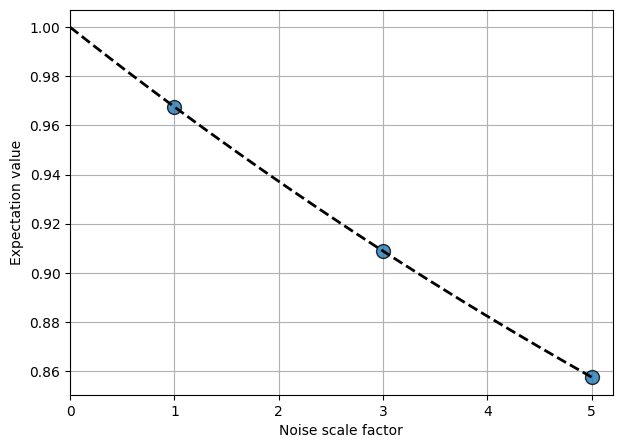
\includegraphics[width=0.7\textwidth]{images/mitiq_plot.png}
    \caption{Zero-Noise Extrapolation (ZNE) workflow implemented using Mitiq. The plot shows the expectation values obtained from noise-scaled circuits using local unitary folding with scale factors of 1.0, 3.0, and 5.0. An exponential extrapolation method is applied to these values to infer the zero-noise limit.}
    \label{fig:zne_mitiq_workflow}
\end{figure}

Combining the equations in step 2 for different extrapolation method, the general expression for $\langle X \rangle^{(0)}$ with $n$ noise levels is:
\begin{equation}
\langle X \rangle^{(0)} = \sum_{i=1}^{n} \gamma_i \langle X \rangle(\lambda_i),
\end{equation}
where the coefficients $\{\gamma_i\}$ are determined by the extrapolation method employed. \\ \\
It is important to note that this error mitigation technique is effective only for short quantum circuits. Consider a quantum circuit with $G$ gates; each gate operates successfully with a probability of $(1-\epsilon)$. Therefore, the maximum probability of errors occurring in the entire circuit can be approximated as $ \sim 1 - (1- \epsilon)^G = G\epsilon + G^2 \epsilon^2/2 + \cdots$. The first term in this expansion corresponds to the contribution from first-order noise terms, and subsequent terms represent higher-order contributions. If $G\epsilon \geq 1$, then the higher-order terms cannot be ignored in Step 2 above. \\ \\
Thus, the zero-noise expectation value of an observable is calculated by artificially amplifying the errors and then extrapolating the curve to estimate the zero-error case. The primary steps in this error reduction process are 1) Noise Amplification and 2) Extrapolation to the zero-noise limit which are discussed in detail below.

\subsection{Noise Scaling}
\subsubsection{Noise Model and Expectation Values}
Noise in quantum systems arises due to environmental interactions, imperfect gate operations, and decoherence. ZNE is applied where the noise is weak, stochastic and time-invariant. Non-stochastic errors arising from multi-qubit gates can be transformed into stochastic errors using techniques such as Pauli twirling \cite{li-PhysRevX.7.021050}. Thus, a general noise channel $\mathcal{N}_\lambda$ can be expressed as a completely positive trace-preserving (CPTP) map:
\begin{equation}
\mathcal{N}_\lambda(\rho) = \sum_i K_i(\lambda) \rho K_i^\dagger(\lambda),
\end{equation}
Where $\{K_i(\lambda)\}$ are Kraus operators representing the Hamiltonian dynamics of the system, satisfying the trace-preserving condition:
\begin{equation}
\sum_i K_i^\dagger(\lambda) K_i(\lambda) = I.
\end{equation}
$\lambda$ is a convenient noise-scaling factor where scaling the noise corresponds to modifying the Kraus operators such that:
\begin{equation}
K_i(\lambda) = f(\lambda) K_i(1),
\end{equation}
where $f(\lambda)$ is a scaling function and $K_i(1)$ is the system without any noise scaling. For example, if $\lambda = 2$, the noise is doubled, which could be achieved by increasing the gate duration or introducing redundant operations. Given this parameterization, the noisy state becomes:
\begin{equation}
\rho_\lambda = \mathcal{N}_\lambda(\rho_0) = \sum_i f(\lambda) K_i(1) \rho_0 f(\lambda) K_i^\dagger(1).
\end{equation}
Substituting the noisy state $\rho_\lambda$ into the expression for the expectation value, $E(\lambda)$ for any observable $\hat{O}$, we get:
\begin{equation}
E(\lambda) = \text{Tr}\left[\hat{O} \cdot \rho_\lambda \right] = \text{Tr}\left[\hat{O} \cdot \sum_i f(\lambda) K_i(1) \rho_0 f(\lambda) K_i^\dagger(1) \right].
\end{equation} \\
By linearity of the trace operation:
\begin{equation}
E(\lambda) = \sum_i f(\lambda)^2 \text{Tr}\left[\hat{O} \cdot K_i(1) \rho_0 K_i^\dagger(1) \right] \tag{11.1}\label{eq:11.1}
\end{equation}
In most practical scenarios, the dependence of $E(\lambda)$ on $\lambda$ can be approximated by a polynomial:
\begin{equation}
E(\lambda) = E_0 + a_1 \lambda + a_2 \lambda^2 + \cdots + a_n \lambda^n + O(\lambda^{n+1}),  
\end{equation}
where $E_0$ is the expectation value at zero-noise and the coefficients $a_1, a_2, \ldots$ depend on the specific noise model.

\subsubsection{Noise Amplification}
The noise level in a quantum circuit can be artificially increased by adjusting gate parameters or adding extra operations \cite{Giurgica_Tiron_2020}, \cite{majumdar2023bestpracticesquantumerror}. It is important to ensure that these amplifying processes are executed within the T1 relaxation and T2 coherence times of the hardware \cite{kandala2019error}. Common techniques for amplifying noise include:
    \begin{enumerate}
        \item \textit{Unitary Gate Folding:} The "unitary folding" method enhances noise resilience by repeating quantum gates. This process increases the circuit depth and effectively scales the noise by a factor of \(2n + 1\). Given a unitary \(U\), the noise-scaled unitary is constructed as given in equation 13. There are two common types of unitary gate folding used in practice:
        \begin{equation}
        U \to U (U^\dagger U)^n
        \end{equation}

        \begin{itemize}
        \item \textit{Local Folding:} Specific gates in the circuit are repeated, effectively increasing the circuit's noise locally. For instance, a single unitary gate $G$ is replaced by $G \cdot G^\dagger \cdot G$. This ensures the operation remains logically equivalent but with amplified noise.
        
        \item \textit{Global Folding:} The entire quantum circuit $C$ is transformed into $C \cdot C^\dagger \cdot C$, where $C^\dagger$ is the circuit's inverse. This method increases the noise uniformly across the entire computation.
        \end{itemize}
                      
        \item \textit{Identity Gate Insertion:} Inserting layers of identity gates throughout the circuit creates idle time for the system to interact with the environment, which can lead to errors. The error rate associated with this method is directly proportional to the number of identity gate layers inserted and the coherence times of the qubit hardware. Similar to unitary folding, identity gates can be inserted between layers of individual gates or after the circuit.

    \item \textit{Pulse Stretching:} Scaling the duration of gates in devices that allow pulse-level control to encourage environmental interference with the qubits, which results in noise. Circuit stretching (pulse stretching) is especially effective for time-invariant noise mechanisms, such as constant-rate amplitude damping, dephasing, or depolarization.
    \end{enumerate}

\subsubsection{Challenges in Noise Scaling}
While noise scaling is conceptually straightforward, its practical implementation poses several challenges:
\begin{itemize}
    \item \textbf{Accuracy of Noise Scaling Factors:} The noise scaling factors ($\lambda$) ($\lambda = 1, 1.5, 2, ...$) must be chosen carefully to ensure proportional scaling of noise. Inaccurate scaling can introduce errors during curve fitting and extrapolation.
    \item \textbf{Hardware Limitations:} On some quantum devices, gate folding or circuit stretching may be limited by the device's native gate operations or coherence times, as stated before. For the same reason, this technique majorly works for quantum circuits with short-depths.
    \item \textbf{Noise Model Dependence:} Noise scaling assumes that there is a predictable relationship between noise levels and expectation values. However, this assumption may not be valid for highly complex or fluctuating noise models. Additionally, the noise must be time-invariant; that is, the time required for significant errors caused by the noise to accumulate is assumed to be much longer than the duration needed to carry out the controlled quantum operations.
\end{itemize}

\subsection{Extrapolating Zero-Noise Limit}
The mathematical framework of ZNE is rooted in the assumption that the expectation value of a quantum observable can be expressed as a power series in the noise parameter $\lambda$ as shown in equation 14:
\begin{equation}
E(\lambda) = E_0 + a_1 \lambda + a_2 \lambda^2 + \cdots
\end{equation}
Where $\lambda$ is the noise scaling parameter, $E(\lambda)$ is the expectation value of the quantum observable in the presence of noise, $a_1, a_2, \ldots$ are coefficients dependent on the specific noise model and quantum circuit; $E_0$ is the zero-noise expectation value to be estimated.
\\ \\
By executing the quantum computation at multiple noise levels $\lambda_1, \lambda_2, \ldots, \lambda_n$, a set of noisy results $\{E(\lambda_1), E(\lambda_2), \ldots, E(\lambda_n)\}$ is obtained. After this noise scaling and obtaining results at multiple noise levels, the next step in ZNE is to estimate the zero-noise value of the observable. This is achieved using classical extrapolation methods. The objective is to determine $E_0$ by fitting the noisy results $\{E(\lambda_i)\}$ to this series and evaluating it at $\lambda = 0$. using classical extrapolation methods \cite{Giurgica_Tiron_2020}.

\subsubsection{Common Extrapolation Techniques}
\begin{enumerate}
    \item \textbf{Linear Extrapolation:} For small noise levels, the power series can be approximated as:
    \begin{equation}
    E(\lambda) \approx E_0 + \sum_{i=1}^{n}a_i \lambda \tag{14.1} \label{eq:14.1}
    \end{equation}
    A straight line is fitted to the data points, and the zero-noise value is obtained by evaluating the fit at $\lambda = 0$. This method is computationally efficient and requires only two or three noise levels, but it assumes that higher-order noise terms are negligible.

    \item \textbf{Polynomial Extrapolation:} For higher-order noise contributions, a polynomial fit of degree $n$ is used to approximate the series:
    \begin{equation}
    E(\lambda) \approx E_0 + a_1 \lambda + a_2 \lambda^2 + \cdots + a_n \lambda^n \tag{14.2} \label{eq:14.2}
    \end{equation}
Polynomial extrapolation is more accurate for complex noise models but requires more data points to fit higher-degree terms reliably. This approach is beneficial when noise behaves non-linearly about the scaling factor.

    \item \textbf{Richardson Extrapolation:} This method constructs a weighted sum of noisy results to cancel out higher-order noise terms. For $n$ noise levels, the zero-noise value is estimated as:
    \[
    E_0 = \sum_{i=1}^{n} \gamma_i E(\lambda_i) \tag{15} \label{eq:15}
    \]
    Where $\gamma_i$ are coefficients determined based on the noise scaling factors. For two noise levels $\lambda_1$ and $\lambda_2$ with $\lambda_2 = c \cdot \lambda_1$, Richardson extrapolation estimates the zero-noise value as:
    \[
    E_0 = \frac{c E(\lambda_1) - E(\lambda_2)}{c - 1}. \tag{16} \label{eq:16}
    \]
    For three noise levels $\lambda_1, \lambda_2, \lambda_3$ with $\lambda_3 = c \cdot \lambda_2 = c^2 \cdot \lambda_1$, Richardson extrapolation can be extended to:
    \[
    E_0 = \frac{c^2 E(\lambda_1) - c E(\lambda_2) + E(\lambda_3)}{c^2 - c}. \tag{16.1} \label{eq:16.1}
    \]
    Richardson extrapolation is especially valuable when a predictable scaling relationship between noise levels exists; it is also the most commonly used method.

    \item \textbf{Poly-Exponential Extrapolation:} Poly-exponential extrapolation combines polynomial fitting and exponential decay to estimate the zero-noise limit for quantum computations. It assumes that the expectation value \( E(\lambda) \) can be modeled as:
    \[
    E_{\text{poly-exp}}(\lambda) = a \pm e^{z(\lambda)}, \quad z(\lambda) = z_0 + z_1 \lambda + \dots + z_d \lambda^d, \tag{17} \label{eq:17}
    \]
    Poly-exponential extrapolation is particularly effective for capturing complex noise behaviors that exhibit both polynomial and exponential characteristics; it is well-suited for systems with non-linear noise scaling.

    \item \textbf{Exponential Extrapolation:} A special case of the more general poly-exponential method, it assumes that the expectation value \( E(\lambda) \) decays exponentially with the noise scaling factor \( \lambda \):
    \[
    E(\lambda) = A e^{-\lambda / \tau} \tag{18} \label{eq:18}
    \]
    By fitting the noisy data to this exponential model, the zero-noise value \( E(0) \) can be extrapolated as \( A \), which corresponds to the intercept of the fitted curve. Using a logarithmic transformation simplifies the fitting process into a linear regression problem:
    \[
    \ln E(\lambda) = \ln A - \frac{\lambda}{\tau}. \tag{18.1} \label{eq:18.1}
    \]

    \item \textbf{Double Exponential Extrapolation:} This method generalizes exponential extrapolation by assuming a sum of two exponential terms to account for multiple noise processes:
    \[
    E(\lambda) = A_1 e^{-\lambda / \tau_1} + A_2 e^{-\lambda / \tau_2}.
    \]
    For small \( \lambda \), the model can be approximated as:
    \[
    E(\lambda) \approx (A_1 + A_2) - \lambda \left( \frac{A_1}{\tau_1} + \frac{A_2}{\tau_2} \right).
    \]
    The zero-noise value \( E(0) = A_1 + A_2 \) is obtained by fitting the noisy data to this model using numerical optimization.
    
\end{enumerate}

Linear extrapolation is suitable when only two or three noise levels are available, whereas polynomial and Richardson extrapolation benefit from additional data points. Polynomial and Richardson methods are preferred for non-linear or higher-order noise effects, while linear extrapolation is adequate for simpler noise models. Polynomial extrapolation involves greater computational cost due to curve fitting, whereas Richardson extrapolation is computationally efficient but assumes proportional noise scaling.


\subsubsection{Limitations of Extrapolation}

Although extrapolation methods provide a practical approach to estimating the zero-noise value, they are not without limitations:
\begin{itemize}
    \item \textbf{Accuracy of Noise Scaling:} Uncontrolled errors in the noise scaling process can introduce inaccuracies in the extrapolated results.
    \item \textbf{Overfitting:} Polynomial extrapolation, when applied with a high degree, may overfit the data and result in unreliable predictions.
    \item \textbf{Assumptions on Noise Models:} Extrapolation assumes a well-behaved relationship between the expectation value and noise level, which may not hold for all noise types.
\end{itemize}

Despite the limitations of noise scaling and extrapolation techniques, zero-noise extrapolation is a robust method for mitigating noise effects in NISQ devices. ZNE is straightforward, scalable, and resource-efficient, making it applicable to various quantum simulations and hybrid quantum algorithms \cite{app-bhattacharjee2024}, \cite{app-halder2023development}. This project further explores the impact of ZNE through its implementation on an efficient SU2 ansatz using Qiskit.


\section{Practical Implementation}
This section details an experiment that we conducted on IBM Quantum computers to test the efficiency of Zero Noise Extrapolation. The code is available on \href{https://github.com/RishwiBT/Quantum-Error-Suppression-mitigation-and-correction/blob/main/ZNE%20Code/Final_QEC_Project_code.ipynb}{GitHub}. ZNE can only be used in experiments that measure the expectation value of an observable. Using IBM Qiskit version 1.3, the main goal is to measure the expectation value of the $ZZZZZZZ.....Z = Z^{\otimes n}$ observable for arbitrary short-depth quantum circuit, in our case, the efficient SU2 circuit \cite{ibm_efficientSU2}.

\subsection{The Implementation Process}
\subsubsection*{1. Noise Amplification:}
    
    \begin{itemize}
        \item \textit{Efficient SU2 Quantum Circuit:} SU(2) stands for the special unitary group of degree 2; its elements are 2×2 unitary matrices with determinant 1, such as the Pauli rotation gates. The EfficientSU2 circuit consists of layers of single-qubit operations spanned by SU(2) and CX entanglement gates. This heuristic pattern can be used to prepare trial wave functions for variational quantum algorithms or classification circuits for machine learning. 
        
        \item \textit{Mirroring the Circuit:} In this experiment, we apply \textbf{Global Folding} where we append the above circuit with its mirror image as mentioned in section 2.2.2. This is equivalent to introducing noise by applying $UU^\dagger = I$ to n qubits initialized in $|0\rangle$ state.         
    \end{itemize}

    \subsubsection*{2. Execution and Extrapolation:}
    \begin{itemize}
        \item \textit{Transpiling the circuit:} After composing the circuit, running it on an actual quantum device needs a transpiled circuit \cite{ibm_transpilation}. Transpilation is rewriting a given input circuit to match a specific quantum device's topology and ISA (instruction set architecture).
        
        \item \textit{Estimating the $Z^\otimes n$ observable:} After successfully building the transpiled circuit, the next step is calculating the Z observable expectation value without and with ZNE error mitigation. ZNE error mitigation is an in-built class in Qiskit that will implement varied noise factors and extrapolate the expectation value. The results are obtained using different extrapolation techniques - linear, polynomial, exponential; and are used to plot and compare the expectation values.
    \end{itemize}

    \subsubsection*{3. Expected Results}
    \begin{itemize}
        \item Because we started with the $|0\rangle ^{\otimes n}$ state and applied $UU^\dagger$ to it, we expect that the output after application of $UU^\dagger$ will remain $|0\rangle ^{\otimes n}$ on which measuring $Z^\otimes n$ should give expectation value 1 in an ideal scenario. However, we will see that the obtained expectation value is lower due to noise/errors.
    
        \item We will also see that when ZNE is applied, it will precisely infer the zero-noise limit expectation value (equal to 1). 
    \end{itemize}

\subsection{Results}
The results, shown in Figure 1, illustrate the varying effectiveness of different extrapolation methods in reducing noise and improving the accuracy of expectation values. Linear extrapolation, although computationally simple, did not demonstrate any significant improvement compared to the unmitigated results. On the other hand, polynomial extrapolation of degree 2 showed a slight improvement, indicating its ability to account for some higher-order noise contributions. Exponential extrapolation provided a notable enhancement, effectively modeling the decay of noise effects and bringing the results closer to the ideal value. Finally, double exponential extrapolation showed the best results, accurately capturing complex noise behaviors and producing results closest to the ideal expectation value. These observations highlight the importance of selecting an appropriate extrapolation method based on the noise complexity and the desired accuracy level.

 \begin{figure*}[t!]
        \subfloat[ZNE with Linear Extrapolation]{%
            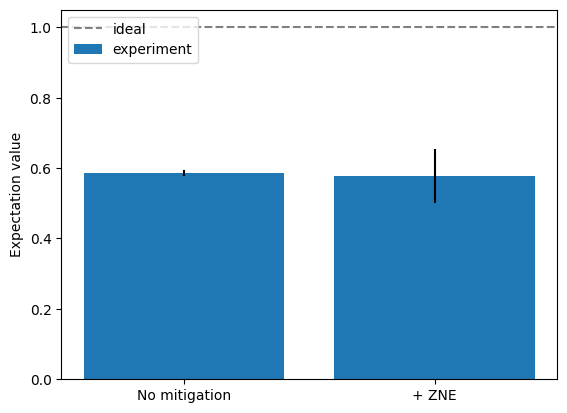
\includegraphics[width=.48\linewidth]{images/linear.png}%
            \label{fig:linear_extrapolation}%
        }\hfill
        \subfloat[ZNE with degree-2 Polynomial Extrapolation]{%
            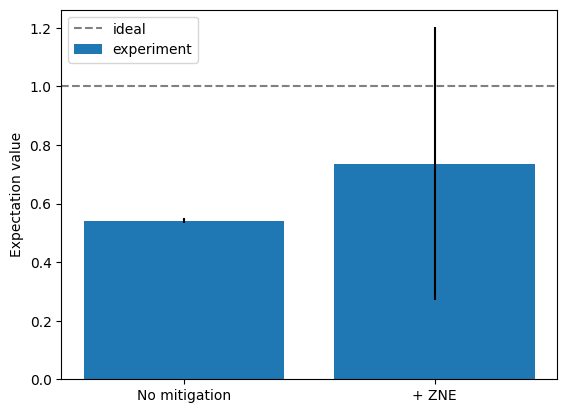
\includegraphics[width=.48\linewidth]{images/polynomial_degree_2.png}%
            \label{fig:polynomial_degree_2}%
        }\\
        \subfloat[ZNE with Exponential Extrapolation]{%
            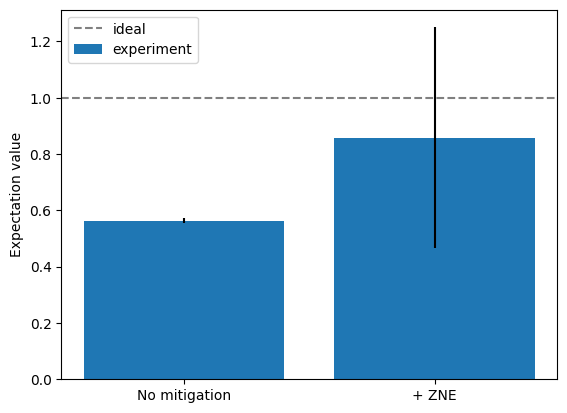
\includegraphics[width=.48\linewidth]{images/exponential.png}%
            \label{fig:exponential_extrapolation}%
        }\hfill
        \subfloat[ZNE with Double-Exponential Extrapolation]{%
            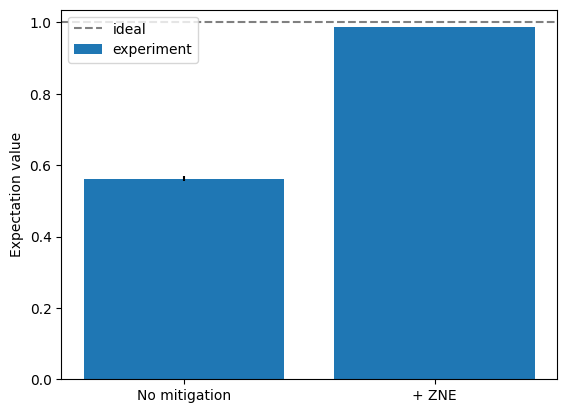
\includegraphics[width=.48\linewidth]{images/double_exponential.png}%
            \label{fig:double_exponential_extrapolation}%
        }
    \caption{Comparison of expectation values with no mitigation and ZNE using a) Linear, b) Polynomial, c) Exponential, d) Double-Exponential extrapolation. Double exponential method achieves results closest to the ideal value}
    \label{fig:fig}
\end{figure*}



\subsection{Error Bounds and Confidence Intervals}
Estimating the uncertainty in the extrapolated zero-noise value is crucial to ensure its reliability. Error bounds help quantify the reliability of ZNE and highlight potential sources of inaccuracies. Although the finer details are found in statistical studies, here we summarize the key points:
\begin{itemize}
    \item Using statistical methods, such as least-squares fitting or weighted regression, to estimate error bounds for the extrapolated value.
    \item Calculating confidence intervals for $E_0$ using bootstrapping techniques, particularly when working with limited data points.
    \item Reporting both the extrapolated value and its associated uncertainty to provide a comprehensive assessment of computation accuracy.
\end{itemize}


\section{Conclusion}
This paper explores the ZNE technique as a prominent error mitigation strategy for noisy intermediate-scale quantum devices. ZNE provides a practical approach to enhancing computational accuracy by utilizing noise scaling and classical extrapolation techniques without additional quantum resources. The article examines its mathematical foundations, which include linear, polynomial, Richardson, exponential, and double exponential extrapolation methods.

The experimental results demonstrate that the choice of extrapolation method significantly affects the effectiveness of ZNE. The exponential and double exponential extrapolation methods are more effective than others, with double exponential fitting achieving the highest accuracy by modeling complex noise decay behaviors.

These findings underscore the importance of understanding noise characteristics and selecting appropriate extrapolation techniques to attain the desired accuracy in quantum computations. As quantum hardware advances, ZNE emerges as a versatile and resource-efficient tool for mitigating noise effects in quantum algorithms. Future research could focus on combining ZNE with other error mitigation strategies, such as Parameterized Error Cancellation (PEC), Parameterized Error Amplification (PEA), and adaptive noise scaling \cite{mod-hysRevResearch.3.033098}, \cite{mod-PhysRevA.104.052607}, \cite{mod-10313621}, as well as exploring its applications in larger-scale quantum systems \cite{app-bhattacharjee2024}, \cite{app-halder2023development}.

Ultimately, ZNE plays a critical role in bridging the gap between current hardware limitations and the requirements for practical, error-mitigated quantum computing, bringing us closer to realizing the full potential of quantum technologies.


\section{Acknowledgement}
We wish to express our gratitude to Dr. Daniel Lidar for providing a strong foundation in the Quantum Error Correction classes, where we explored all the essential tools and technologies currently used in practical quantum applications. \\
This project was a collaborative effort, with both students contributing equally. We shared the workload for the literature review and content writing. Rishwi handled the implementation on Qiskit hardware, while Pranavi took care of the LaTeX formatting and final editing. \\
The authors would also like to acknowledge the use of Grammarly to enhance the writing style.

\addcontentsline{toc}{section}{References}
\bibliographystyle{IEEEtran}
\bibliography{bibliography/references}

% \section{References}
% \begin{thebibliography}{9}
% \bibitem{zurek} Zurek, W. H. (2002). \textit{Decoherence and the Transition from Quantum to Classical—Revisited}. Los Alamos Science, 27, 2-3.
% \bibitem{giurgica} Giurgica-Tiron, T. et al. (2021). \textit{Digital Zero Noise Extrapolation for Quantum Error Mitigation}. arXiv:2005.10921.
% \bibitem{kandala} Kandala, A. et al. (2019). \textit{Error mitigation extends the computational reach of a noisy quantum processor}. Nature, 567, 491–495.
% \end{thebibliography}

\end{document}
